\chapter{Einleitung}
IT-Sicherheit wird in der Software Entwicklung ein immer wichtigeres  Thema. In Abbildung \ref{FIG:statistic-ausgaben-it-sicherheit} ist der Anstieg der Ausgaben für IT-Sicherheit zu sehen. Dieser ist in den vergangen Jahren kontinuierlich gestiegen und auch in der Zukunft sollen die Ausgaben im Jahr 2025 im Vergleich zu 2020 um 57.5\% steigen. Das zeigt das vielen Unternehmen die IT-Sicherheit immer wichtiger wird. Die dafür anfallenden Kosten sollen aber natürlich trotzdem immer möglichst gering bleiben.
DevOps ist mittlerweile eine verbreitete und viel genutzte Entwicklungsmethode (siehe Abb. \ref{FIG:devops-important}) um den Entwicklungsprozess zu beschleunigen und somit auch Kosten zu sparen. Um den It-Sicherheitsaspekt einfach in die Softwareentwicklung zu integrieren wurde so DevSecOps erschaffen. Der Prozess vereint DevOps mit Sicherheitsverfahren. \cite{security-model}
Zwei der größten Plattformen für DevOps sind GitHub und Azure DevOps. GitHub liefert GitHub Actions und Azure DevOps bietet Azure Pipelines um Operationen aus dem DevOps Prozess zu automatisieren. Diese Frage ist welches Tool den DevSecOps Prozess am besten integriert um sichere Software zu erstellen.


\begin{figure}[H]
	{\caption{Ausgaben für IT-Sicheheit in Deutschland in den Jahren 2017 bis 2020 und Prognose bis 2025 (in Milliarden Euro)}
		\label{FIG:statistic-ausgaben-it-sicherheit}}
	{
\includegraphics[width=1\textwidth]{figures/statistic-ausgaben-it-sicherheit.png}}
\end{figure}

\chapter{Was bedeutet DevSecOps}

\section{Zusammenfassung DevOps}
DevOps setzt sich aus den Begriffen \glqq Development \grqq{}(Entwicklung) und \glqq Operations \grqq{}(Vorgänge) zusammen. Die traditionelle Trennung von Entwicklung und Softwarebetrieb führt oft zu Interessenskonflikten. Entwickler wollen stetig die Software verbessern, der Betrieb hingegen will Änderungen vermeiden um die Stabilität des System zu gewährleisten. \cite{git-ops} Beim Einsetzten von  DevOps wird das Entwickeln und den Betrieb von Software näher zusammengeführt. Es entsteht ein Softwareentwicklungs-Prozess, in dem man durch Automatisierungen das Bauen, Testen und Bereitstellen von Software beschleunigen will. Dies erreicht man durch Praktiken wie Continous Integration, Continous Delivery, Continous Deployment, automatisiertes Teste, Infrastructure-as-Code und automatische Veröffentlichungen. Durch die automatische Bereitstellung der Anwendung und der Infrastruktur entsteht eine schnellere Bereitstellung, bessere Softwarequalität und auch schon mehr IT-Sicherheit. \cite{dev-ops} Außerdem steht DevOps auch für offene Zusammenarbeit, Kommunikation, Transparenz, Eingestehen von Fehlern und das gemeinsame lösen von Problemen, um Konflikte im Team zu vermeiden. Man will schnelles Feedback ermöglichen und somit das Risiko der Softwareentwicklung minimieren. DevOps beschränkt sich also nicht nur auf technische Hilfsmittel sondern bietet eine Kultur um den Entwicklungsprozess immer weiter zu verbessern.\cite{git-ops}

\section{Sicherheitsrisiken und Chancen mit DevOps}
DevOps alleine bringt einige Herausforderungen zum Thema Softwaresicherheit mit sich. Oft wird Sicherheit für Entwicklungsgeschwindigkeit aufgegeben. Gründe dafür sind, das bei der Umstellung bestehende Sicherheitsmethodiken nicht mir DevOps integrierbar waren oder haben nicht in den Agilen Prozess gepasst.
Typischerweise werden dann Sicherheitstests erst am Ende mit der fertig entwickelten Software durchgeführt. Dadurch ist das Sicherheitsteam komplett vom DevOps Prozess ausgeschlossen.

Je schneller die Releaseitegrationen werden, desto weniger Aufwand wird in die Sicherheit gesteckt. Da mit DevOps geänderter Code auch schnell produktiv eingesetzt wird, hat das Entwicklungsteam meistens zu wenig Zeit um die Änderungen sicherheitsrelevant zu Prüfen. Dies bietet dann eventuell neue Angriffsmöglichkeiten oder Risiken in der Software.
Ein weiteres Risiko ist, dass das neue Einsetzten von Cloud Computing neue Sicherheitsmaßnahmen fordert, welche zusätzlich berücksichtigt werden müssen.


DevOps liefert aber auch Chancen um IT-Sicherheit in den Entwicklungsprozess zu integrieren.
Feste, Zentrale und Standardisierte Bereitstellungspipelines helfen dem Security Team einen besseren Blick über die Anwendung und wie diese erstellt wird zu bekommen. Hier können dann verschieden Sicherheitsaspekte in die Pipeline eingebaut werden. DevOps bietet hier also schon einige Möglichkeiten IT-Sicherheit schon in den DevOps Prozess zu integrieren. \cite{grey}

\section{Definition von DevSecOps}
Der Begriff DevSecOps baut auf den Prinzipien und Praktiken von DevOps auf und fügt den Sicherheitsaspekt in der Entwicklung noch weiter in den Vordergrund. Es ist also eine Erweiterung des DevOps Prozesses. Durch DevSecOps soll IT-Security schon vom Start eines Projektes mitgeplant und auch in Bereitstellungsprozess integriert werden. Allerdings reicht es nicht, die Sicherheitsaspekte nur in frühere Phasen der Entwicklung zu verschieben. Es soll eine durchgängige Sicherheit durch ständiges Dazulernen und Verbessern des Sicherheitsprozesses im ganzen Projekt und dessen Bereitstellung entstehen. \cite{grey}
Am Ende ist also das ganze Team für die Applikationssicherheit verantwortlich und Probleme sollen auch im Team angegangen werden. \cite{devsecops-techniques}

Eine technologische Rahmenbedingungen für DevSecOps ist das Bedürfnis für die Automatisierung von Sicherheitsaufgaben im Entwicklungsprozess. Das Einbauen von Sicherheitschecks in die Bereitstellungspipelines reduzieren Zeit und Kosten von Fehlern, die sonst manuell gefunden werden müssen. Zusätzlich wird die IT-Sicherheit in den kompletten Lebenszyklus einer Software integriert und somit können auch Entwickler ohne viel Wissen über IT-Security einfach die automatischen Pipelines nutzen. Das selbe gilt auch für die Bereitstellung der Infrastruktur. Infrastrucutre as Code muss auch eine sichere und zuverlässige Bereitstellung liefern, um auch hier Sicherheitslücken zu vermeiden. \cite{grey}.

\section{Praktiken von DevSecOps}
DevSecOps muss in verschiedenen Prozessen praktiziert werden, um es auf den ganzen Entwicklungsprozess abzubilden zu können.
In der Planungsphase müssen bei der Risikoanalyse Sicherheitsaspekte berücksichtigt werden und eine passende Strategie für das restliche Projekt erstellt zu können.
Während der Entwicklung helfen statische Code Analyzen und Code Reviews um Probleme zu finden, bevor der Code eingecheckt wurde. Die Produktivität der Entwickler wird dadurch nur minimal eingeschränkt, es können aber schon erste Fehler erkannt und ausgebessert werden.
Nachdem der Code eingecheckt wurde sollten beim Erstellen der Software automatisierte Tests laufen, die feststellen ob es Fehler beim erstellen gibt. Auch Abhänigkeitsanalyzen und Unit Tests sollen kritische Sicherheitsprobleme aufdecken und den verantwortlichen Entwickler benachrichtigen.

Auch die automatisierte Bereitstellung der Infrastrukur ist ein wichtiger Teil, der gesichert sein muss und auch essenzielle Auswirkungen auf das komplette System hat.
Hier sind Themen wie Secrets Management, Configuration Management oder Version Control wichtige Aspekte, um die man sich kümmern muss.\cite{grey}

\cite{security-model} entwickelte ein Security Model um Sicherheitspraktiken in die komplette Infrastrukturbereitstellung zu bringen. Nachdem ein statischer Analyse Security Scanner den Terraform Code analysiert hat, wird der dieser in einen verschlüsselten Objektspeicher in der Cloud ausgeführt. Hier werden alle benötigten SSH Schlüssel automatisch runter geladen. Die von Terraform erstellten IP-Adressen der Infrastruktur werden an Ansible gesendet welches die erstellten Server dann konfiguriert. Am Ende werden alle Geheimnisse von den Servern gelöscht. So wird eine sichere Bereitstellung der Infrastruktur gewährleistet.

Wenn die Applikation dann auf einer Testumgebung installiert wurde sollen statische und dynamische Security Tests laufen. Auch automatisierte Attacken sollen Bestandteil des automatischen Testzyklus sein.
Im Livebetrieb der Software sollen regelmäßig automatische Sicherheitschecks und Überwachung des Systems stattfinden, um einen Einblick in den Datenverkehr zu bekommen und eventuell bösartige Benutzerverhalten aufdecken zu können.
DevSecOps wirkt sich auch auf das Personal aus. Es muss in einem Entwicklungsteam immer \glqq Security Chanpions\grqq \cite{grey} geben. Diese sollen besonders Wissen über IT-Sicherheit und dem Entwicklungszyklus haben, um wie auch schon bei DevOps ein funktionsübergreifendes Team zu schaffen.
Auch ein regelmäßiges Training der Entwickler und Bereitstellung wichtiger Tools führen dazu das IT-Sicherheit nicht nur nebenbei läuft sondern zu einer Geisteshaltung die das ganze Unternehmen durchdringt.
Es gibt also viele verschiedene Praktiken, die man in die Softwareentwicklung integrieren kann und soll.

\section{DevSecOps Engineer als Beruf}
Viele Stoßen beim Einführen von DevSecOps in ihren Entwicklungsprozess auf Herausforderungen. Das sind teilweise hohe Kosten, schon bestehende solide Organisationsstrukturen oder kultureller Widerstand von Entwicklern. Eine Möglichkeit dagegen ist es, einen DevSecOps Spezialisten anzustellen. Dieser kann die Transformation der Arbeitskultur vorantreiben und beschleunigen. Der Experte kann die Einführung verschiedener DevSecOps Tools übernehmen und mit seinem Wissen schneller Sicherheitsintegrationen in zum Beispiel bestehende Pipelines durchführen. \cite{grey}
Auch DevOps wird oft als Jobbeschreibung verstanden. Als \glqq DevOps Engineer\grqq arbeitet man in verschiedenen DevOps-Teams und -Abteilungen. Diese haben vor allem die Aufgabe genannte Praktiken von DevOps durchzuführen. \cite{dev-ops}
Ein DevSecOps Engineer setzt auf den Beruf eines DevOps Engineers mit dem Fokus auf IT-Security auf. Er muss ein tiefes Verständnis mitbringen wie sich IT-Security auf die einzelnen Phasen der Entwicklung und das Endprodukt auswirkt. Seine Aufgaben sind es, die automatisierten Sicherheitspraktiken in die Pipeline zu implementieren und immer wieder zu überprüfen und aktuell zu halten. Man sollte also gut in jeden Schritt der Softwareentwicklung integriert sein. Er muss sich natürlich aber auch mit normalen DevOps Prozessen und Prinzipien auskennen. Außerdem sollte er versuchen die restlichen skeptischen Teammitglieder überzeugen, das die Sicherheitspraktiken wichtig sind und die Entwicklungsgeschwindigkeit nicht verlangsamen. Um für einen solchen Job angestellt zu werden helfen verschiedene Zertifikate über DevSecOps Engineering. \cite{Cobb2019-lq}


\chapter{DevSecOps mit Azure DevOps}

\chapter{DevSecOps mit Github Actions}

\section{Zusammenfassung der Sicherheitsfunktionen}
\begin{figure}[H]
	{\caption{Architektur von GitHub für DevSecOps Prozess}
		\label{FIG:devsecops-in-github}}
	{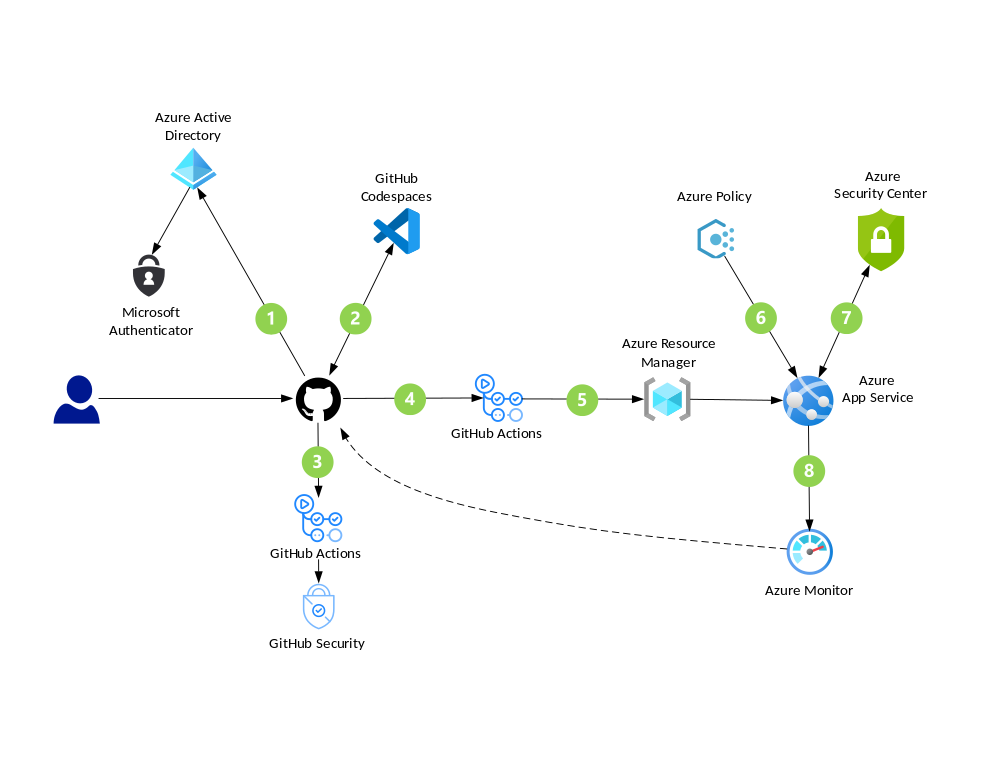
\includegraphics[width=1\textwidth]{figures/devsecops-in-github.png}}
\end{figure}
GitHub bietet mit GitHub Security ein Konzept DevSecOps abzubilden und in den Entwicklungsprozess zu integrieren. Der Aufbau ist in Abbildung \ref{FIG:devsecops-in-github} zu sehen und im folgendem Abschnitt grob beschrieben.

Wenn Entwickler auf GitHub Ressourcen zugreifen, müssen sie eine Authentifizierung über eine Azure Actice Directory durchlaufen. Hier wird eine sichere kennwortlose  FIDO2-Authentifizierung verwendet, die nach aktuellen Standards entspricht. \cite{fido2}
Mit GitHub Codespaces können Entwickler auf vordefinierte Entwicklungsumgebungen in Containern zugreifen, die mit erforderlichen Erweiterungen für Sicherheitsscans ausgestattet sind.
Durch GitHub Actions können automatisch Codierungsfehler und Schwachstellen durch automatische Scans beim Einchecken ermittelt werden.
Außerdem können die Bildartefakte direkt in einen Azure App Service deployed werden.
Durch Pull Requests können weitere automatisierte Tests ausgeführt werden. Außerdem bietet es eine gute Platform um Code Reviews durchzuführen.
Microsoft Defender for Cloud identifiziert Attacken in bereitgestellten Projekten
Durch den Azrure Monitor können regelmäßig das Verhalten der laufenden Software überwacht evaluiert und Auffälligkeiten automatisch gemeldet werden.\cite{devsecops-github}

\section{Github Security Lab}
Mit dem GitHub Security Lab bietet die Plattform ein Portal, auf dem sie versuchen User zu inspirieren und es ihnen ermöglichen leichter sichere Open Source Software zu implementieren. 
Auf der Plattform können Schwachstellen von großen, wichtigen Open Source Projekten berichtet werden. Das Portal koordiniert dann die Offenlegung der Schwachstellen mit den Sicherheitsteam der betroffenen Projekte. Es werden zusätzlich verschiedene Analysen mit CodeQL, einer semantischen Code-Analyse-Engine durchgeführt um die Sicherheitsforschung für Open Source Projekte zu vergrößern. Zusätzlich werden Common Vulnerabilities und Exposures in einer Datenbank gesammelt.
Außerdem werden viele Forschungen, Tutorials, Artikel oder Konferenzen veröffentlicht und der Community bereitgestellt.
Es werden auch mit dem so genannten \glqq CodeQL Bug Bounty program\grqq immer wieder Prämien ausgeschrieben, um Sicherheitsforschung in der Community zu verstärken. Die Plattform bietet also über die technischen Funktionen von GitHub hinaus, die Möglichkeit für Entwickler sich über IT-Sicherheit zu vernetzten, zu lernen oder sich an der Sicherheitsforschung für Open Source Projekte zu beteiligen. \cite{github-securitylab}


\chapter{Vergleich von Github Actions und Azure DevOps}

\chapter{Fazit}
Github ist am Aufstreben blablabla